
\begin{enumerate}
\item Draw a quadrilateral in the Cartesian plane, whose vertices are $(-4,5), (0,7), (5,-5)$ and $(-4,-2)$. Also, find its area.
\item The base of an equilateral triangle with side $2a$ lies along the y-axis such that the mid-point of the base is at the origin. Find vertices of the triangle.
\item Find the distance between $P(x_1,y_1),Q(x_2,y_2)$ when:
\begin{enumerate}[label=(\roman*)]
\item $PQ$ is parallel to the y-axis.
\item $PQ$ is parellel to the x-axis.
\end{enumerate}
\item Find the point x-axis, which is equidistant from the points $(7,6)$ and $(3,4)$.
\item Find the slope of a line, which passes through the origin, and the mid-point of the line segment joining the points $P(0,-4)$ and $B(8,0)$.
\item Without using the Pythagoras thorem, show that the points $(4,4), (3,5)$ and $(-1,-1)$ are the vertices of a right angled triangle.
\item Find the slope of the line, which makes an angle of 30° with the positive  direction of y-axis measured anticlockwise.
\item Find the value of $x$ for which the points $(x,-1), (2,1)$ and $(4,5)$ are collinear.
\item Without using distance formula, show that points $(-2,-1), (4,0), (3,3)$ and $(-3,2)$ are the vertices of the parallelogram.
\item Find the angle between the x-axis and the line joining the points $(3,-1)$ and $(4,-2)$.
\item The slope of a line is double of the slope of another line. If tangent of the angle between them is $\frac{!}{3}$, find the slopes of the lines.
\item A line passes through $(x_1,y_1)$ and $(h,k)$. If slope of the line is m, show that:
\item $k-y_1= m(h-x_1)$
\item If three points $(h,0), (a,b)$ and $(0,k)$ lie on a line, show that $\frac{a}{h}+\frac{b}{k}=1$.
\item Consider the following population and year graph  \figref{fig:10.10}, find the slope of the line $AB$ and using it, find what will be the population in the year $2010$?
\begin{figure}[ht]
\centering
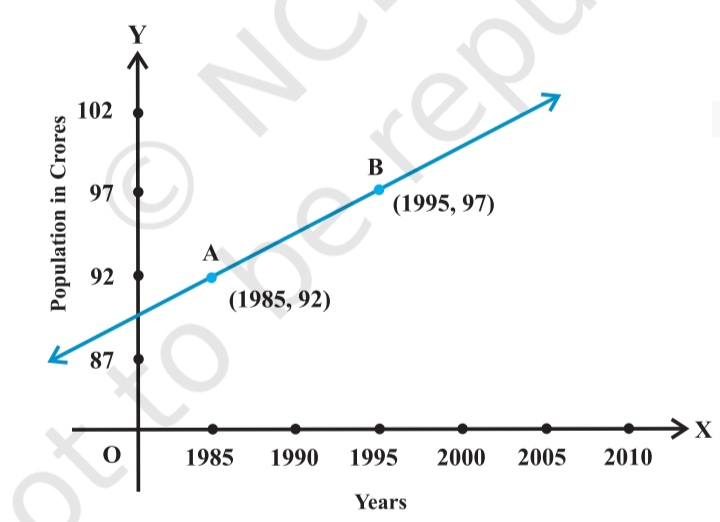
\includegraphics[width=\columnwidth]{chapters/11/figs/10.10.png}
\caption{10.10}
\label{fig:10.10}
\end{figure}
\end{enumerate}

